% Microeconomics*
% Final Exam covering Chs. 1-4, 6-9
% Administered May 2026
%----------------------------------------------
\documentclass[12pt]{exam}

\usepackage{setspace}
\setstretch{1.15}
\nopointsinmargin
\pointformat{}

\usepackage{problemset}

\usepackage[margin=1in]{geometry}

\noprintanswers
%\printanswers

\begin{document}

\FontEasyRead

\Heading
{Microeconomics*}
{Cumulative Test}
{75 Minutes, 100 points plus 10 potential bonus points.
  Annotated (by you) version of my cheat-sheet permitted, but no other resources.
  Answer all multiple-choice questions by selecting the best answer.
  Answer all short-response questions clearly, using correct reasoning.
Show all work for math problems. Do not skip any problems - there is always potential for partial credit.}

%%%%%%%%%%%%%%%%%%%%%%%%%%%%%%%%%%%%%%%%%%%%%%%%%%%%%%
\section*{Part I: Multiple Choice (1 point each)}

\begin{questions}

  \begin{mcquestion}[1]
    Opportunity cost is best defined as:
    \begin{choices}
      \choice The monetary cost of a decision only
      \CorrectChoice The value of the best forgone alternative
      \choice Total accounting profit
      \choice The price paid for a good
    \end{choices}
  \end{mcquestion}

  \begin{mcquestion}[1]
    The law of demand states that:
    \begin{choices}
      \choice As price increases, quantity demanded increases
      \CorrectChoice As price increases, quantity demanded decreases
      \choice Demand is unrelated to price
      \choice Supply determines demand
    \end{choices}
  \end{mcquestion}

  \begin{mcquestion}[1]
    A market is in equilibrium when:
    \begin{choices}
      \choice Quantity demanded exceeds quantity supplied
      \choice Price is changing rapidly
      \CorrectChoice Quantity demanded equals quantity supplied
      \choice Firms earn zero revenue
    \end{choices}
  \end{mcquestion}

  \begin{mcquestion}[1]
    If income increases and a good is normal, demand will:
    \begin{choices}
      \choice Decrease
      \choice Stay the same
      \CorrectChoice Increase
      \choice Become perfectly inelastic
    \end{choices}
  \end{mcquestion}

  \begin{mcquestion}[1]
    Price elasticity of demand measures:
    \begin{choices}
      \choice How price responds to supply changes
      \CorrectChoice Responsiveness of quantity demanded to price changes
      \choice Total revenue changes only
      \choice Cost changes in production
    \end{choices}
  \end{mcquestion}

  \begin{mcquestion}[1]
    If demand is elastic, a price increase will:
    \begin{choices}
      \choice Increase total revenue
      \CorrectChoice Decrease total revenue
      \choice Leave revenue unchanged
      \choice Eliminate demand
    \end{choices}
  \end{mcquestion}

  \begin{mcquestion}[1]
    Economic profit differs from accounting profit because it:
    \begin{choices}
      \choice Ignores revenue
      \CorrectChoice Includes opportunity costs
      \choice Ignores costs
      \choice Equals total revenue
    \end{choices}
  \end{mcquestion}

  \begin{mcquestion}[1]
    Diminishing marginal returns occurs when:
    \begin{choices}
      \choice Output increases proportionally with inputs
      \CorrectChoice Each additional unit of input adds less output than the previous
      \choice Costs decrease as output increases
      \choice Firms shut down
    \end{choices}
  \end{mcquestion}

  \begin{mcquestion}[1]
    Fixed costs are:
    \begin{choices}
      \choice Costs that vary with output
      \CorrectChoice Costs that do not vary with output
      \choice Always zero in the long run
      \choice Equal to marginal cost
    \end{choices}
  \end{mcquestion}

  \begin{mcquestion}[1]
    In the short run, a firm should shut down if:
    \begin{choices}
      \choice Price is below average total cost
      \CorrectChoice Price is below average variable cost
      \choice Revenue is positive
      \choice Marginal cost equals price
    \end{choices}
  \end{mcquestion}

  \begin{mcquestion}[1]
    Marginal cost is:
    \begin{choices}
      \choice Total cost divided by quantity
      \CorrectChoice The cost of producing one additional unit
      \choice Fixed cost per unit
      \choice Average revenue
    \end{choices}
  \end{mcquestion}

  \begin{mcquestion}[1]
    A profit-maximizing firm in perfect competition produces
    at a level where:
    \begin{choices}
      \choice Price equals total cost
      \choice Marginal revenue is zero
      \CorrectChoice Price equals marginal cost
      \choice Average cost is minimized
    \end{choices}
  \end{mcquestion}

  \begin{mcquestion}[1]
    A binding price ceiling causes:
    \begin{choices}
      \choice Surplus
      \CorrectChoice Shortage
      \choice No effect
      \choice Increased equilibrium price
    \end{choices}
  \end{mcquestion}

  \begin{mcquestion}[1]
    A binding price floor above equilibrium price causes:
    \begin{choices}
      \choice Shortage
      \CorrectChoice Surplus
      \choice Market equilibrium
      \choice Zero production
    \end{choices}
  \end{mcquestion}

  \begin{mcquestion}[1]
    If supply increases, equilibrium price will generally:
    \begin{choices}
      \choice Increase
      \CorrectChoice Decrease
      \choice Stay constant
      \choice Become infinite
    \end{choices}
  \end{mcquestion}

  \begin{mcquestion}[1]
    With goods where demand is inelastic, consumers tend to:
    \begin{choices}
      \choice Avoid price changes entirely
      \CorrectChoice Bear more of the tax burden
      \choice Shift supply curves
      \choice Eliminate scarcity
    \end{choices}
  \end{mcquestion}

  \begin{mcquestion}[1]
    A firm is a price taker when:
    \begin{choices}
      \choice It sets market price
      \CorrectChoice It cannot influence market price
      \choice It is a monopoly
      \choice It has no costs
    \end{choices}
  \end{mcquestion}

  \begin{mcquestion}[1]
    Total revenue is:
    \begin{choices}
      \choice Price minus quantity
      \CorrectChoice Price times quantity
      \choice Marginal cost times quantity
      \choice Fixed cost plus variable cost
    \end{choices}
  \end{mcquestion}

  \begin{mcquestion}[1]
    A shift in supply can be caused by:
    \begin{choices}
      \choice A change in price
      \CorrectChoice A change in input costs or manufacturing technology
      \choice A change in quantity demanded
      \choice A change in equilibrium only
    \end{choices}
  \end{mcquestion}

  \begin{mcquestion}[1]
    In our two-good model, utility maximization occurs when:
    \begin{choices}
      \choice Total utility is zero
      \CorrectChoice Marginal utility per dollar is equal across both goods
      \choice Income is maximized
      \choice Marginal utility is the same for both goods
    \end{choices}
  \end{mcquestion}

  %%%%%%%%%%%%%%%%%%%%%%%%%%%%%%%%%%%%%%%%%%%%%%%%%%%%%%
  \section*{Part II: Short Answer (10 points each)}

  \begin{shortanswer}[10]{2.5in}
    A sudden 25\% increase in the price of refrigerators causes quantity
    demanded to fall sharply at first, but later recover. Explain what's happening
    in terms of short-run and long-run price elasticity of demand.  Are refrigerators
    durable or non-durable goods?
  \end{shortanswer}
  \begin{solution}
    Short-run demand is more elastic (consumers make-do with their old refrigerators); long-run
    demand is more inelastic as consumers adjust (and their old fridges wear out). Refrigerators
    are durable goods.
  \end{solution}


  \begin{problem}[15]{4in}
    Assuming typical supply and demand curves, fill in each box with the effect on
    equilibrium price and quantity. Use these codes:

    \begin{itemize}
      \item Price up, same, down, ambiguous: P-U, P-S, P-D, P-A
      \item Quantity up, same, down, ambiguous:  Q-U, Q-S, Q-D, Q-A
    \end{itemize}

    The easy box has been filled-in for you. ``Ambiguous'' means the outcome could be up, same, or
    down, depending on the relative magnitudes and/or elasticities.

    \vspace{0.5cm}

    \begin{center}
      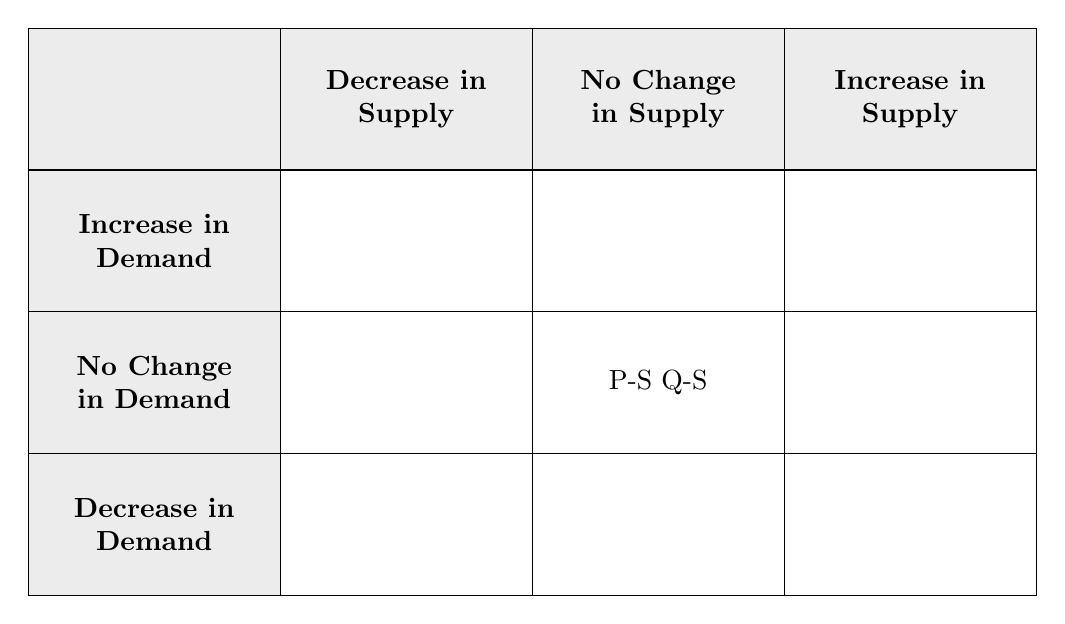
\begin{tikzpicture}[
          every node/.style={draw, align=center, minimum height=1.8cm},
          header/.style={font=\bfseries, fill=gray!15},
          cell/.style={minimum width=3.2cm},
          rowlabel/.style={minimum width=3.2cm, font=\bfseries, fill=gray!15}
        ]

        % Top row (column headers)
        \node[header, minimum width=3.2cm] at (0,0) {};
        \node[header, cell] at (3.2,0) {Decrease in\\Supply};
        \node[header, cell] at (6.4,0) {No Change\\in Supply};
        \node[header, cell] at (9.6,0) {Increase in\\Supply};

        % Row 1
        \node[rowlabel] at (0,-1.8) {Increase in\\Demand};
        \node[cell] at (3.2,-1.8) {};
        \node[cell] at (6.4,-1.8) {};
        \node[cell] at (9.6,-1.8) {};

        % Row 2
        \node[rowlabel] at (0,-3.6) {No Change\\in Demand};
        \node[cell] at (3.2,-3.6) {};
        \node[cell] at (6.4,-3.6) {P-S Q-S};
        \node[cell] at (9.6,-3.6) {};

        % Row 3
        \node[rowlabel] at (0,-5.4) {Decrease in\\Demand};
        \node[cell] at (3.2,-5.4) {};
        \node[cell] at (6.4,-5.4) {};
        \node[cell] at (9.6,-5.4) {};

      \end{tikzpicture}
    \end{center}

    Sketch here as needed:

  \end{problem}

  %%%%%%%%%%%%%%%%%%%%%%%%%%%%%%%%%%%%%%%%%%%%%%%%%%%%%%
  \section*{Part III: Math Problems (10 points each)}

  \begin{problem}[15]{3in}
    Given the CPI-U table:

    \begin{center}
      \renewcommand{\arraystretch}{1.4}
      \setlength{\tabcolsep}{12pt}

      \begin{tabular}{|>{\centering\arraybackslash}p{3cm}|>{\centering\arraybackslash}p{5cm}|}
        \hline
        \textbf{Year} & \textbf{CPI-U Annual Average Index} \\
        \textbf{} & \textbf{(1982--1984 = 100)} \\
        \hline
        2020 & 258.811 \\
        \hline
        2021 & \entryblank \\
        \hline
        2022 & 292.655 \\
        \hline
        2023 & \entryblank \\
        \hline
        2024 & 319.799 \\
        \hline
      \end{tabular}
    \end{center}

    Given:
    \begin{itemize}
      \item Inflation from 2020 to 2021 = 4.69802\%
      \item Average annual inflation from 2020 to 2023 = 5.76852\%
    \end{itemize}

    Find the missing CPI values.
  \end{problem}
  \begin{solution}
    Apply inflation formula:
    \[
      CPI_{2021} = 258.811 \times (1.0469802)
    \]
    and compound for 2023.
  \end{solution}


  \begin{problem}[15]{4in}
    Given a firm's marginal revenue and marginal cost functions:
    \[
      MR(q) = 100 - 4q, \quad MC(q) = 20 + q
    \]

    \begin{itemize}
      \item Find its profit-maximizing \( q \)
      \item At that $q$, find price using \( P(q) = 100 - 2q \)
      \item Find total revenue
      \item Given a cost function of \( C(q) = 20q + 0.5q^2 \), compute the firm's profit
    \end{itemize}
  \end{problem}
  \begin{solution}
    Set \( MR = MC \):
    \[
      100 - 4q = 20 + q \Rightarrow q = 16
    \]
    \[
      P = 100 - 32 = 68
    \]
    \[
      TR = 68 \cdot 16 = 1088
    \]
    \[
      C = 320 + 128 = 448
    \]
    Profit = 640
  \end{solution}
  \begin{problem}[10]{2in}
    A product price rises from 10 to 12 and quantity demanded falls from 50 to 40. Compute price elasticity of demand.
  \end{problem}
  \begin{solution}
    % midpoint elasticity
    $E = \frac{(40-50)/45}{(12-10)/11} = \frac{-10/45}{2/11} = -2.44$
  \end{solution}

  \begin{problem}[10]{2in}
    A firm has cost function $TC = 50 + 10q + q^2$. Find marginal cost and average cost.
  \end{problem}
  \begin{solution}
    $MC = 10 + 2q,\quad AC = \frac{50}{q} + 10 + q$
  \end{solution}

  \begin{problem}[10]{3in}
    Given demand $P = 60 - Q$ and cost $TC = 20 + 10Q$, find profit-maximizing output and price.
  \end{problem}
  \begin{solution}
    $TR = (60-Q)Q = 60Q - Q^2$ $\rightarrow$ $MR = 60 - 2Q$
    $MC = 10$
    Set $MR = MC: 60 - 2Q = 10$ $\rightarrow$ $Q = 25$ $\rightarrow$ $P = 35$
  \end{solution}

  %%%%%%%%%%%%%%%%%%%%%%%%%%%%%%%%%%%%%%%%%%%%%%%%%%%%%%
  \section*{Bonus Question - 10 points}

  \begin{shortanswer}[10]{3in}
    What is one concept from microeconomics that you think helps
    explain real-world pricing or decision-making most clearly to you?
  \end{shortanswer}
  \begin{solution}
    Answers vary.
  \end{solution}

\end{questions}

\end{document}
